% ===========================================================================================
%                                           |                                               |
% -------------------------------------- SECTION -------------------------------------------|
%                                           |                                               |
% ===========================================================================================
\section{Robot equations of motion}
\subsection{Forward and inverse dynamics}
\subsection{The Newton-Euler formulation of the inverse dynamics}

Extension for floating base robots with flexible joints and links have been presented elsewhere \cite{Khalil2017GeneralDynamicAlgorithm}
% The kinematics forward recursion
% The dynamics backward recursion
\subsection{Composition of the kinematics and dynamics}
%bsection{Basics of robot system identification}
%bsubsection{Kinematic calibration}
%bsubsection{Inertial parameter identification}
% For fixed based robots
% For floating base robots

% ===========================================================================================
%                                           |                                               |
% -------------------------------------- SECTION -------------------------------------------|
%                                           |                                               |
% ===========================================================================================
\section{Robot proprioception}
\subsection{Definition}
\subsection{Human and robot proprioception}
\subsection{A sensor suite for robot proprioception}

% ===========================================================================================
%                                           |                                               |
% -------------------------------------- SECTION -------------------------------------------|
%                                           |                                               |
% ===========================================================================================
\section{State-of-the-art Gradient Descent}
\subsection{Fundamentals}
\subsection{Momentum gradient descent}
\subsection{ADAM gradient descent}
\subsection{AMS gradient descent}

% ===========================================================================================
%                                           |                                               |
% -------------------------------------- SECTION -------------------------------------------|
%                                           |                                               |
% ===========================================================================================
\section{Fundamentals of graph theory}

\subsection{Definition of a graph}
A graph $\mathcal{G} = \left(\mathcal{V}, \mathcal{E}\right)$ is a mathematical construct the represents the interconnections between the elements of a system. These elements are represented as a set $ \mathcal{V}=\left\lbrace v_i\right\rbrace^n_{i=1}$ of $n$ \emph{nodes} (also called \emph{vertices}) and their connections are depicted as a set of \emph{edges} $ \mathcal{E}= \left\lbrace e_i\right\rbrace^m_{i=1} \subseteq \mathcal{V} \times \mathcal{V} $. Note that it is possible that an edge connects a node to itself, in which case the edge defines a self loop.
% ---
%\begin{figure}[th!]
%	\begin{center}
%		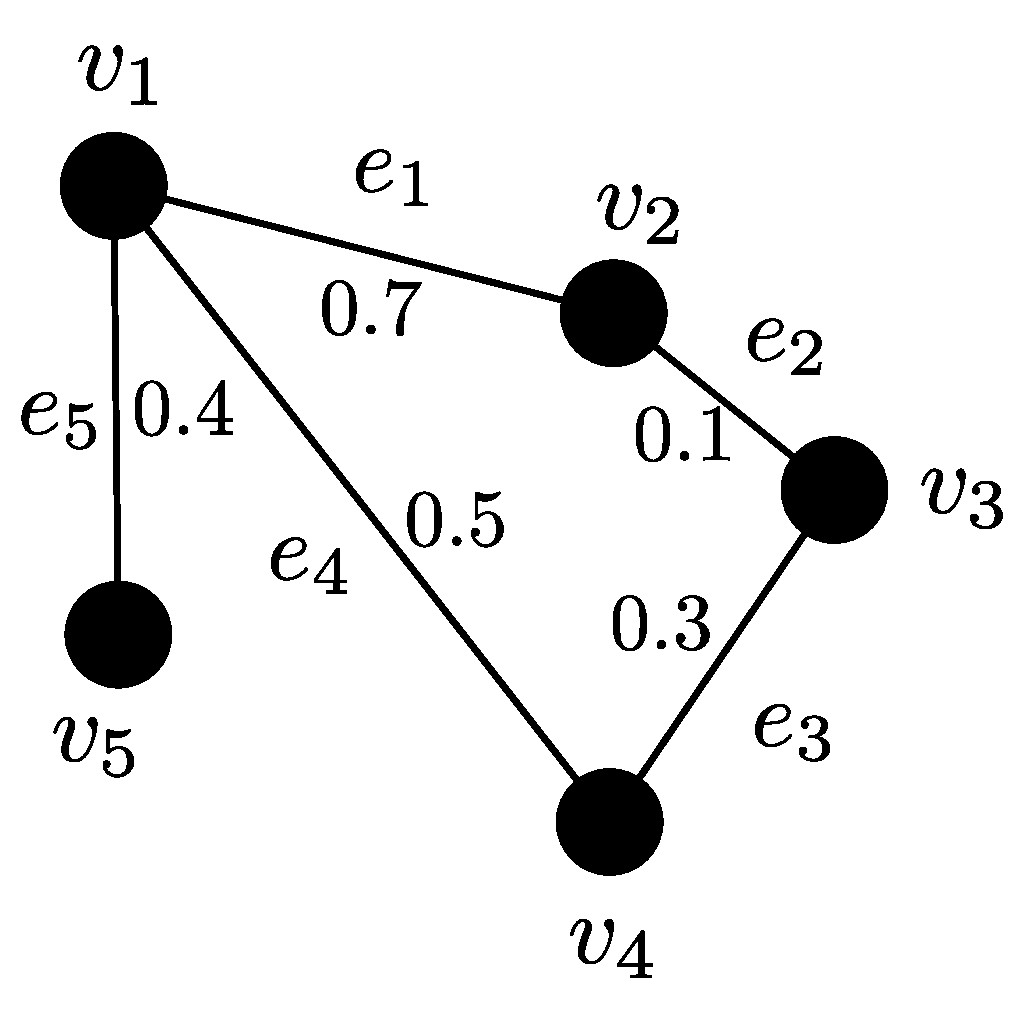
\includegraphics[width=0.5\textwidth]{example_graph.pdf}
%		\caption{Example graph.}
%		\label{fig:example_graph}
%	\end{center}
%\end{figure}
% ---
\begin{figure*}[!h]
	\centering	
	\hspace*{\fill}
	\begin{subfigure}[t]{0.32\textwidth}
		\subcaption{}
		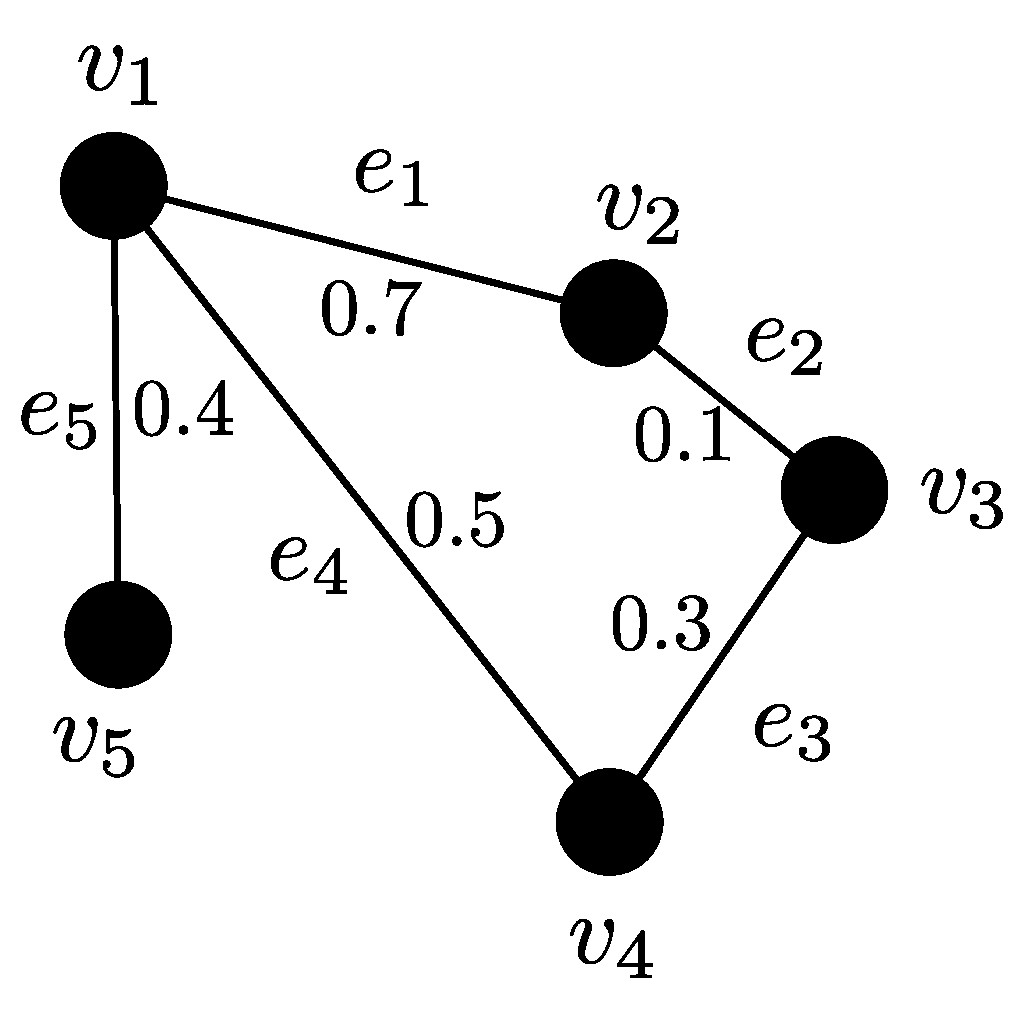
\includegraphics[width=\textwidth]{example_graph.pdf}
		\label{fig:example_graph}
	\end{subfigure}	
	\hfill
	\begin{subfigure}[t]{0.32\textwidth}
		\subcaption{}
		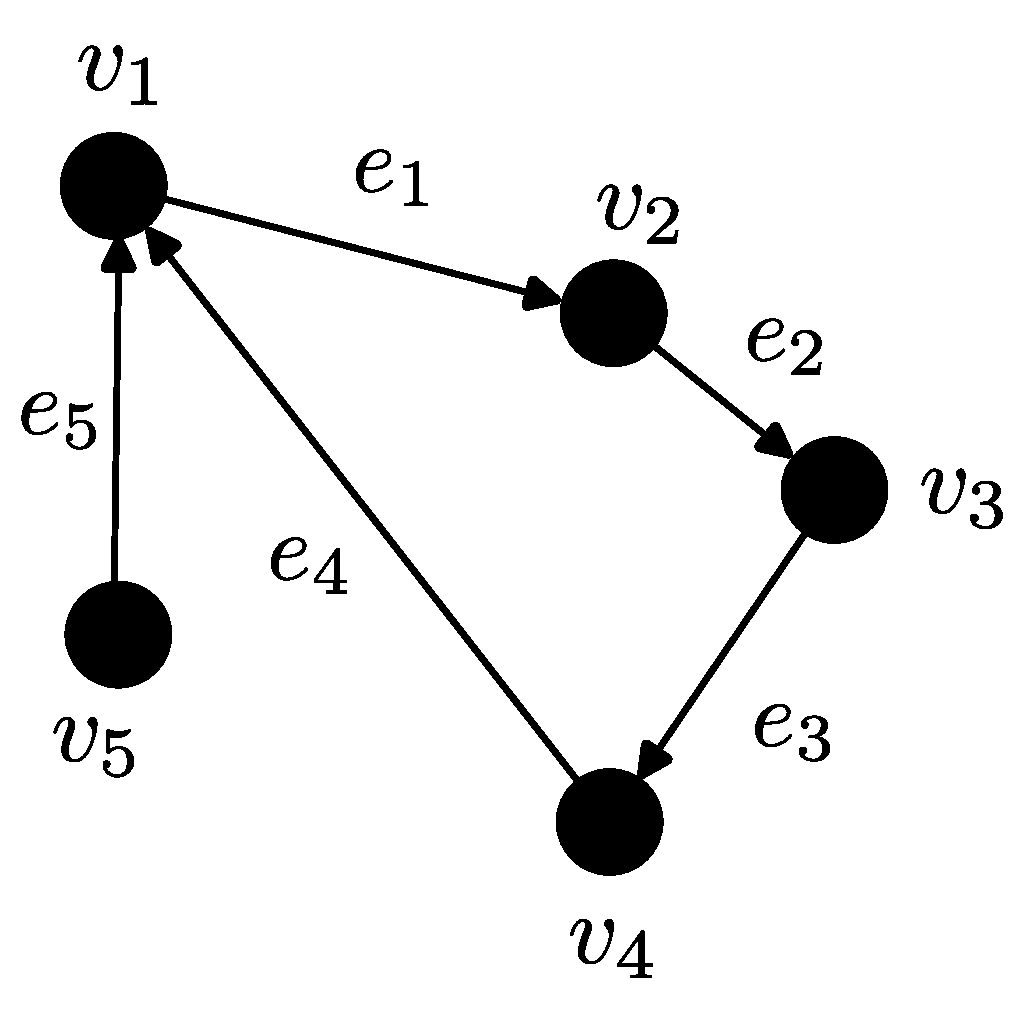
\includegraphics[width=\textwidth]{example_digraph.pdf}
		\label{fig:example_digraph}
	\end{subfigure}
	\hspace*{\fill}	
	\caption[] {\label{fig:graph_examples} \textbf{Two basic types of graphs}. (\subref{fig:example_graph}) An undirected and (\subref{fig:example_digraph}) a directed graph.}
\end{figure*}

%\begin{figure*}[!h]
%	\centering	
%	\hspace*{\fill}
%	\begin{subfigure}[t]{0.32\textwidth}
%		\subcaption{}
%		\includegraphics[width=\textwidth]{f6a_phantomx_hexapod.pdf}
%		\label{fig:phantomx_robot}
%	\end{subfigure}	
%	\hfill
%	\begin{subfigure}[t]{0.32\textwidth}
%		\subcaption{}
%		\includegraphics[width=\textwidth]{f6b_phantomx_pi_graph_kinematics.pdf}
%		\label{fig:phantomx_pigraph_kin_clusters}
%	\end{subfigure}
%	\hfill
%	\begin{subfigure}[t]{0.32\textwidth}
%		\subcaption{}
%		\includegraphics[width=\textwidth]{f6c_phantomx_morphology.pdf}
%		\label{fig:phantomx_morphology}
%	\end{subfigure}	
%	\hspace*{\fill}
%	\\
%	\hspace*{\fill}
%	\begin{subfigure}[t]{0.96\textwidth}
%		\subcaption{}
%		\includegraphics[width=\textwidth]{f6d_phantomx_morphology_errors_offline.pdf}
%		\label{fig:phantomx_morphology_errors_offline}
%	\end{subfigure}	
%	\hspace*{\fill}
%	\\
%	\hspace*{\fill}
%	\begin{subfigure}[t]{0.96\textwidth}
%		\subcaption{}
%		\includegraphics[width=\textwidth]{f6e_phantomx_morphology_errors_online.pdf} 		
%		\label{fig:phantomx_morphology_errors_online}
%	\end{subfigure}	
%	\hspace*{\fill}	
%	\caption[] {\label{fig:hexapod_simulated_results} \textbf{The hexapod robot}. (\subref{fig:phantomx_robot}) the PhantomX hexapod robot with its IMUs (red spheres), (\subref{fig:phantomx_pigraph_kin_clusters}) the kinematics graph $\mathcal{G}^{\mathcal{K}}_\pi$, (\subref{fig:phantomx_morphology}) the learned kinematic structure, errors in the estimated body structure via (\subref{fig:phantomx_morphology_errors_offline}) offline learning and (\subref{fig:phantomx_morphology_errors_online}) online learning (blue: difference rotation errors $\bar{\delta}~[\text{rad}]$, orange: sensor-to-sensor vector errors $\bar{\tilde{r}}~[\text{m}]$).}
%\end{figure*}
Two nodes $i$ and $j$ are said to be \emph{adjacent} if there is an edge $e$ connecting them. Similarly, the edge $e$ connecting the nodes is called \emph{incident} to $i$ and $j$. For example, the nodes $v_1$ and $v_4$ in Fig.~\ref{fig:example_graph} are adjacent to each other and the edge $e_4$ is incident to both nodes. The number of edges that are incident to a node is the \emph{degree} of the vertex. 

A \emph{path} represents a potential sequence of edges connecting any two given nodes. The number of edges determines the \emph{length} of the path. A graph is said to be \emph{connected} if there is at least one path between every pair of nodes; otherwise, it is labeled \emph{disconnected}. A \emph{cycle} constitutes a path comprising a minimum of three edges, where the initial and final vertices are identical, and no vertices are repeated in between. Lastly, a graph is \emph{complete} if there exists a path connecting every pair of nodes. Notice that the maximum number of edges in an undirected graph with $n$ nodes is $n(n-1)/2$

An \emph{undirected} graph lacks any specified direction assigned to its edges, meaning the connections between nodes are bidirectional. On the other hand, a \emph{directed} graph, commonly referred to as a \emph{digraph}, introduces directionality to its edges. In a directed graph, each edge has an explicit direction, indicating a one-way flow from one node to another. This directional information adds an extra layer of complexity to the relationships within the graph, as opposed to the bidirectional nature of edges in an undirected graph.

%A graph (or network) is a structure  that expresses the relationships between a set of vertices $ \mathcal{V}=\left\lbrace v_i\right\rbrace^m_{i=1}$ via a set of edges $ \mathcal{E}\subseteq \mathcal{V} \times \mathcal{V} $ with weights $ \bm{W}: \mathcal{V} \times \mathcal{V}\to \mathbb{R}_+$. Known as the weighted adjacency matrix, $ \bm{W} $ serves as the algebraic representation of $\mathcal{G}$.
A \emph{weighted} graph $ \mathcal{G}\big(\mathcal{V},\mathcal{E},\bm{W}\big) $ associates numerical value, a weight, to each edge. The weights with weights $ \bm{W}: \mathcal{V} \times \mathcal{V}\to \mathbb{R}_+$ express some quantitative measure such as distance, cost, time, or any other relevant metric depending on the context of the graph. Unlike an unweighted graph, where edges simply represent connections between nodes, a weighted graph provides additional information about the relationships between nodes. For a weighted graph, the \emph{strength} of a vertex corresponds to the sum of the edge weights associated with it.


\subsection{Algebraic representation of a graph}
A graph with $n$ vertices can be represented as a square $n\times n$ matrix $\bm{A}$. This algebraic representation is called the \emph{adjacency matrix} and depicts the graph's connectivity pattern; that is, the elements of the matrix indicate whether pairs of vertices $\left(i,j\right)$ are adjacent or not in the graph. Formally,
the elements of a \emph{binary} adjacency matrix $\bm{A}$ are determined as follows
% ---
\begin{equation}
	\left(\bm{A}\right)_{i,j} =
	\begin{cases}
		1 & \text{if and edge connects nodes $i$ and $j$}\\
		0 & \text{otherwise}.
	\end{cases}
\end{equation}
% --
By extension, a \emph{weighted} adjacency matrix $\bm{W}$ denotes a weighted connection for some of the $\left(i,j\right)$ entries, i.e $\left(\bm{W}\right)_{i,j} \in \mathbb{R}_+$. If the graph is undirected, the adjacency matrix is symmetric, which implies that $\bm{A}=\bm{A}^\intercal$ and $\bm{W}=\bm{W}^\intercal$respectively. Note, however, that for the case of digraphs, the adjacency matrix is not necessarily symmetric. To illustrate this, refer to the graph in Fig.~\ref{fig:example_graph}, the corresponding binary and weighted adjacency matrices are
% ---
\begin{equation*}
	\bm{A} = \begin{bmatrix}
		0 & 1 & 0 & 1 & 1\\
		1 & 0 & 1 & 0 & 0\\
		0 & 1 & 0 & 1 & 0\\
		1 & 0 & 1 & 0 & 0\\
		1 & 0 & 0 & 0 & 0\\
	\end{bmatrix}
\end{equation*} 
% ---
and
\begin{equation*}
	\bm{W} = \begin{bmatrix}
		0 & 0.7 & 0 & 0.5 & 0.4\\
		0.7 & 0 & 0.1 & 0 & 0\\
		0 & 0.1 & 0 & 0.3 & 0\\
		0.5 & 0 & 0.3 & 0 & 0\\
		0.4 & 0 & 0 & 0 & 0\\
	\end{bmatrix}.
\end{equation*} 
% ---
Similarly, for the digraph in Fig.~\ref{fig:example_digraph}, the adjacency matrix is
% ---
\begin{equation*}
	\bm{A}_D = \begin{bmatrix}
		0 & 1 & 0 & 0 & 0\\
		0 & 0 & 1 & 0 & 0\\
		0 & 0 & 0 & 1 & 0\\
		1 & 0 & 0 & 0 & 0\\
		1 & 0 & 0 & 0 & 0\\
	\end{bmatrix}.
\end{equation*} 
% ---
Notice that unless there are self loops in the graph, the main diagonal of an adjacency matrix contains only zero entries. Two other important matrices related to a graph $ \mathcal{G} $ are the degree matrix $ \bm{D}: (\bm{D}_{ii})=\sum_{j=1}^{m} w_{ij} $, a diagonal matrix whose entries are the sum of the rows of $ \bm{W} $, and the combinatorial graph Laplacian (CGL), defined as $ \bm{L}_\text{CGL} = \bm{D} - \bm{W} $ \cite{Mateos2019ConnectingdotsIdentifying}.

\subsubsection{The normalized adjacency matrix} 
The normalized adjacency matrix, defined as
% ---
\begin{equation}
	\mathbfcal{W} = \bm{D}^{-\frac{1}{2}} \bm{W} \bm{D}^{-\frac{1}{2}},
\end{equation}
% --- 
is particularly employed in spectral graph theory \cite{Spielman2012Spectralgraphtheory} and related analyses. Normalization helps account for variations in node degrees and provides a more balanced representation of the graph structure. One common application is in spectral clustering algorithms \cite{VonLuxburg2007tutorialspectralclusteringa}, where the normalized adjacency matrix is used to compute eigenvectors and eigenvalues, aiding in the identification of clusters or communities within a graph. %It also finds applications in various graph-based machine learning and data mining tasks.

\subsection{Subgraphs and spanning trees}
A \emph{subgraph} $\mathcal{G}_1$ is obtained by selecting a subset of the nodes of another graph $\mathcal{G}$ and a corresponding subset of the edges connecting those nodes. Formally, a graph $\mathcal{G}_1\left(\mathcal{V}_1, \mathcal{E}_1\right)$ is a subgraph of $\mathcal{G}$ if and only if $\mathcal{V}_1 \subseteq  \mathcal{V}$ and $\mathcal{E}_1 \subseteq \mathcal{E}$. This is written $\mathcal{G}_1 \subseteq \mathcal{G}$. One particular subgraph of interest in this work are spanning trees. First, a \emph{tree graph} is a graph that does not contain cycles. Such structure usually depicts a hierarchical arrangement. Consequently, a \emph{spanning tree} $\mathcal{G}_1$ of a graph $\mathcal{G}$ is a subgraph containing all the nodes in $\mathcal{G}$ and whose edges form a tree that defines paths that ensure that all the nodes remain connected. The edges of $\mathcal{G}_1$ are denoted as the branches of the tree. In general, a graph $\mathcal{G}_1$ is said to be a spanning subgraph of $\mathcal{G}$ if and only if $\mathcal{V}_1 = \mathcal{V}$ and $\mathcal{E}_1 \subseteq \mathcal{E}$. It is worth noting that every connected graph has a spanning tree and that there are $n^{n-2}$ distinct spanning trees with $n - 1$ edges on a connected graph with $n$ vertices \cite{West2001Introductiongraphtheory}. Examples of spanning trees are shown in Fig.~\ref{fig:tree_examples}.

\subsubsection{Minimum spanning tree and Kruskal's algorithm}
The minimum spanning tree of an undirected, connected, and weighted graph is the spanning tree whose edge weight sum is less than or equal to that of all other spanning trees \cite{Sefidgarminimumspanningtree}. Kruskal's algorithm \cite{Kershenbaum1972Computingminimumspanning} is the standard method to find th minimum spanning tree of a graph. In this work we use an equivalent concept, the \emph{maximum spanning tree} (MST), which corresponds to the spanning tree with maximum edge weight sum.
% ---
\begin{figure*}[!t]
	\centering	
	\hspace*{\fill}
	\begin{subfigure}[t]{0.32\textwidth}
		\subcaption{}
		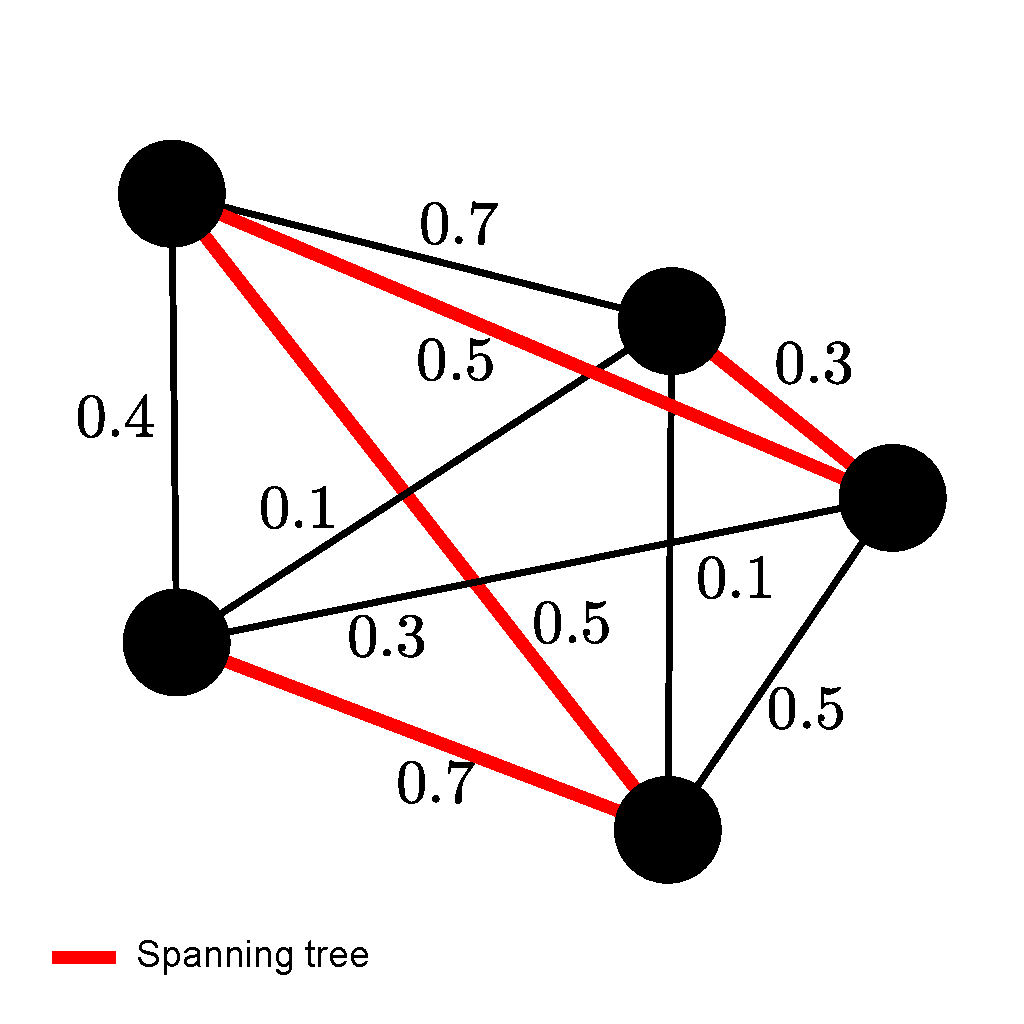
\includegraphics[width=\textwidth]{example_tree_1.pdf}
		\label{fig:example_tree_1}
	\end{subfigure}	
	\hfill
	\begin{subfigure}[t]{0.32\textwidth}
		\subcaption{}
		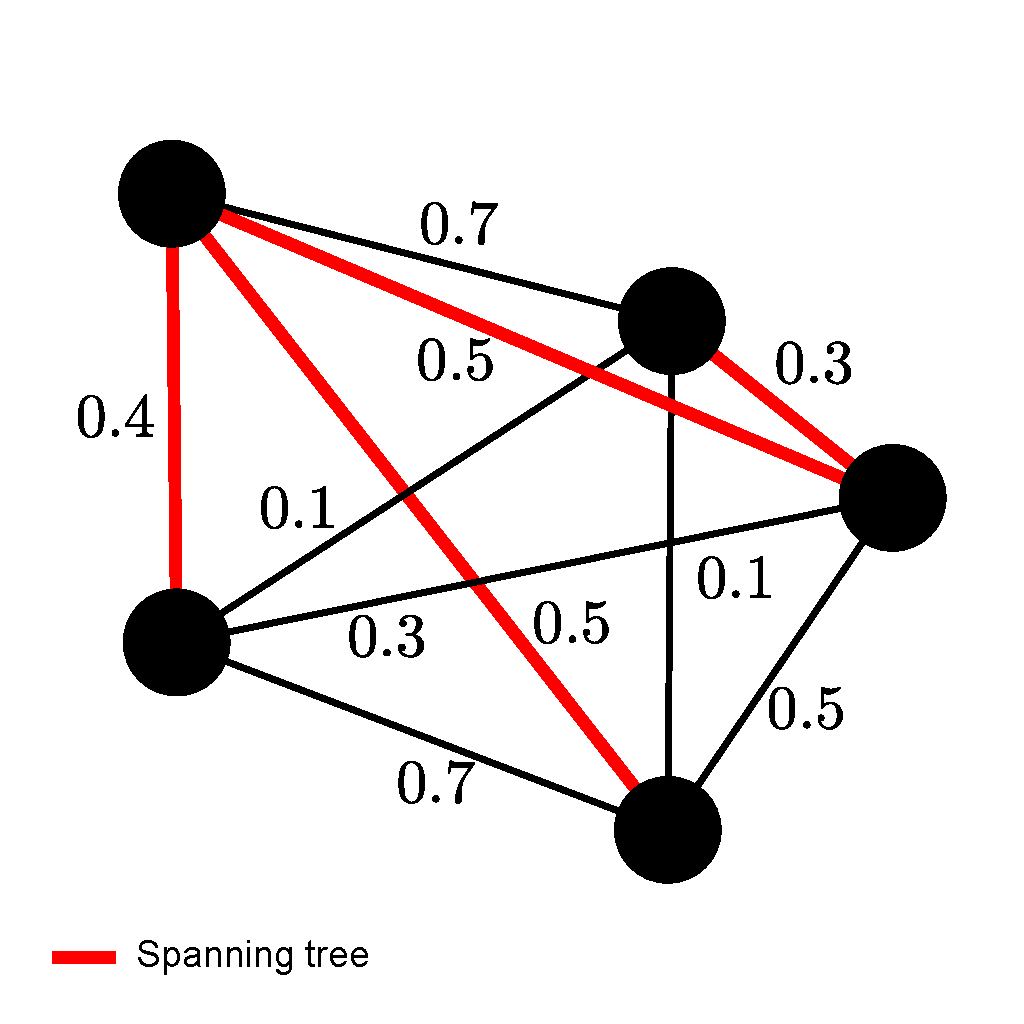
\includegraphics[width=\textwidth]{example_tree_2.pdf}
		\label{fig:example_tree_2}
	\end{subfigure}
	\hfill
	\begin{subfigure}[t]{0.32\textwidth}
		\subcaption{}
		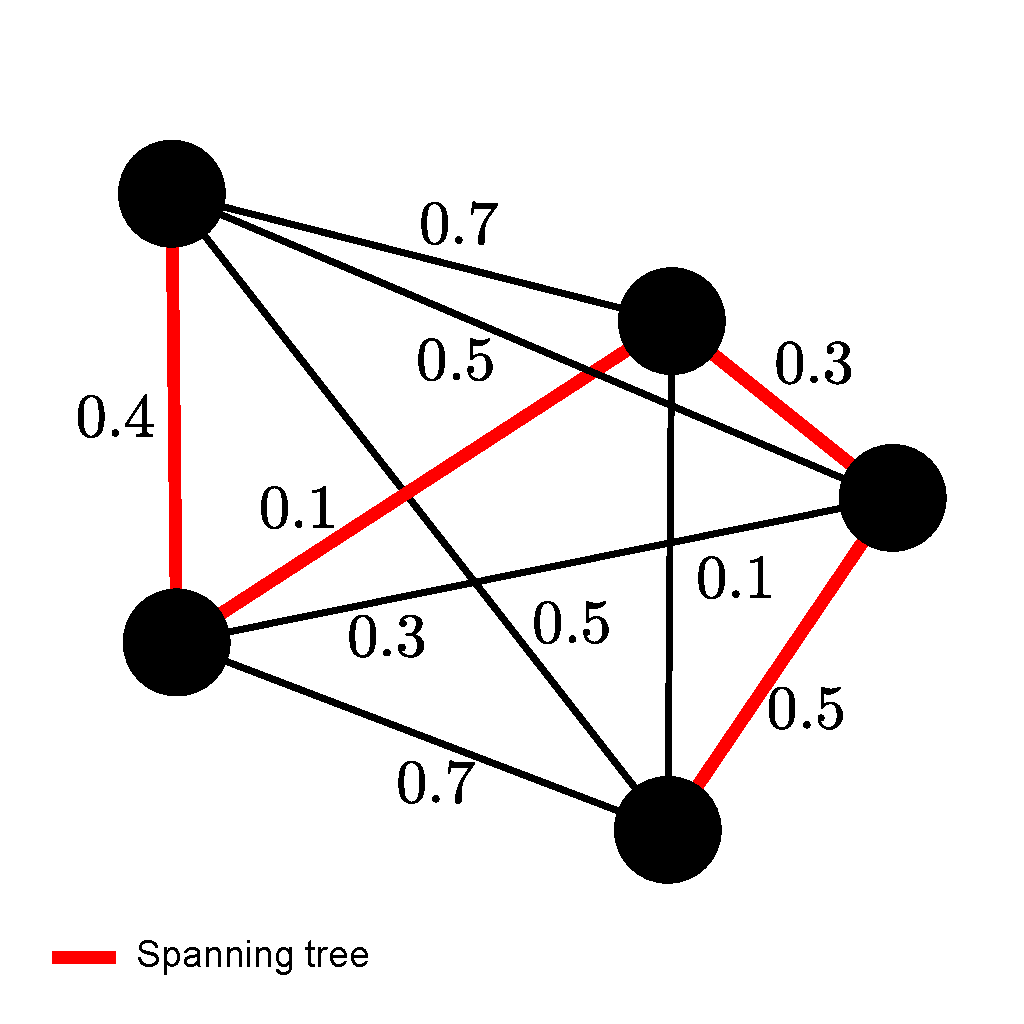
\includegraphics[width=\textwidth]{example_tree_3.pdf}
		\label{fig:example_tree_3}
	\end{subfigure}	
	\hspace*{\fill}	
	\caption[] {\label{fig:tree_examples} \textbf{Different spanning trees for the same graph}.}
\end{figure*}



\subsection{Metrics for graph comparison}
\TODO

% ===========================================================================================
%                                           |                                               |
% -------------------------------------- SECTION -------------------------------------------|
%                                           |                                               |
% ===========================================================================================
\section{Network topology inference}
The process of identifying and visually representing relationships among various elements within a system, based on the available measurements, is termed \emph{network topology inference} (NTI) \cite{Dong2019Learninggraphsdata}. Unveiling the structure of a network or graph through topology learning facilitates the analysis of interactions among entities. 

\subsection{Types connectivity}
%Finding and graphically representing the relationships among the different constituent elements of a system given the available measurements is known as \emph{network topology inference} (NTI) \cite{Dong2019Learninggraphsdata}. By learning the topology of a network/graph, it is possible to reveal a structure that aids in the analysis of the interaction among the entities. As discussed in \cite{Friston2011Functionaleffectiveconnectivity}, one method to represent interaction is via \emph{functional connectivity} (FC), which is an information-theoretic
%measure that characterizes dependencies based on the probability distributions of the observed signals (examples include correlations and mutual information). FC can be further subdivided into non-directed and directed, with the latter being related to statistical causation from the data \cite{Bastos2016tutorialreviewfunctional}. In contrast, \emph{effective connectivity} refers explicitly to the dynamic (state-dependent) influence that one element on the network has on another under a particular network model of causal dynamics; i.e, it refers to coupling or directed causal influence \cite{Park2013Structuralfunctionalbrain}. Exemplary works that use the concepts above can be found in biology\cite{Zhang2017Networkbasedmachine} and neuroscience \cite{Karwowski2019Applicationgraphtheory,Sporns2018Graphtheorymethods}.

\begin{figure*}[!h]
	\centering	
	\hspace*{\fill}
	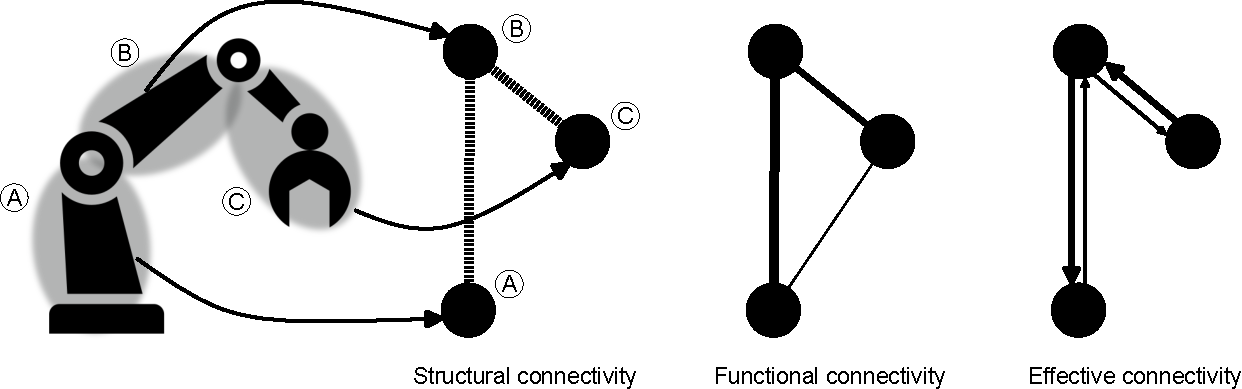
\includegraphics[width=0.9\textwidth]{types_of_connectivity.pdf}
	\hspace*{\fill}	
	\caption[] {\label{fig:types_of_connectivity}\textbf{Types of connectivity.} Every rigid body in the robot represents a node in the graphs.}
\end{figure*}

Often used in the field of neuroscience \cite{Karwowski2019Applicationgraphtheory}, three different types of connectivity are distinguished\cite{Park2013Structuralfunctionalbrain,FaskowitzEdgesbrainnetworks}:

\paragraph*{Structural Connectivity (SC).} Refers to the physical connections between different elements in a network. In the context of neuroscience, it typically involves the anatomical connections between brain regions. It is measured with techniques such as diffusion-weighted imaging (DWI) or diffusion tensor imaging (DTI) are commonly used to infer structural connectivity in the brain.

\paragraph*{Functional Connectivity (FC).} Refers to the statistical dependencies or temporal correlations between the activity of different elements in a network. As explained in \cite{Friston2011Functionaleffectiveconnectivity}, FC is an information-theoretic metric that characterizes dependencies using probability distributions of observed signals. It can be categorized into non-directed and directed forms, with the latter being associated with statistical causation derived from the data \cite{Bastos2016tutorialreviewfunctional}. %FC is often assessed through statistical methods applied to time-series data to identify patterns of correlated activity between different brain regions.

\paragraph*{Effective Connectivity (EC).} Specifically addresses the dynamic, state-dependent influence that one network element has on another within a particular causal dynamics model. Essentially, effective connectivity denotes coupling or directed causal influence \cite{Park2013Structuralfunctionalbrain}. Exemplary applications of these concepts can be observed in the fields of biology \cite{Zhang2017Networkbasedmachine} and neuroscience \cite{Karwowski2019Applicationgraphtheory,Sporns2018Graphtheorymethods}.

To understand the intricate relationships among the three types of connectivity refer to Fig.~\ref{fig:types_of_connectivity}. The figure depicts a simple robot arm as an example. The nodes represent the three links that compose the robot. Regarding SC and FC, a nuanced connection exists, albeit not strictly one-to-one. For example, the SC reflect the physical composition of the body, three bodies connected by two joints (the edges in the SC graph). Sensory signals coming from these bodies might lead to potential functional interactions of varied degree (the edges in the FC graph) that have a foundation on the bodily structure of the robot; yet, it does not ensure their occurrence. Actually, functional relationships can appear even in the absence of direct structural connections, not the light edge between nodes $A$ and $C$ in the FC graph. Moving to EC and FC, the former extends the latter by seeking to model the direction and strength of influence between different elements. While FC identifies statistical associations, EC strives to unveil the underlying causal relationships, the directed edges in the EC graph. In summary, these three connectivity types are interrelated components in the complex landscape of NTI. Structural connections provide the anatomical substrate, functional connections depict statistical dependencies, and effective connections aspire to model causal relationships within the network.


%\redtext{The relationships between SC, FC, and EC in NTI are intricate and multifaceted. Regarding structural and functional connectivity, a nuanced connection exists, albeit not strictly one-to-one. Structural connectivity establishes the anatomical foundation for potential functional interactions, but it doesn't ensure their occurrence. Notably, functional correlations can manifest even in the absence of direct structural connections. Moving to effective connectivity and functional connectivity, the former extends the latter by seeking to model the direction and strength of influence between different elements. While functional connectivity identifies statistical associations, effective connectivity delves deeper, striving to unveil the underlying causal relationships. In summary, these connectivity types are interrelated components in the complex landscape of network topology inference. Structural connections provide the anatomical substrate, functional connections depict statistical dependencies, and effective connections aspire to model causal relationships within the network.} %While these concepts are often explored within the realm of neuroscience, their principles are versatile and applicable to understanding other intricate systems beyond the brain.
%**Relationships:**
%- **Structural and Functional Connectivity:** There is a relationship between structural and functional connectivity, but it's not one-to-one. Structural connectivity provides the anatomical substrate for potential functional interactions, but structural connections do not guarantee functional interactions, and functional correlations can occur in the absence of direct structural connections.
%
%- **Effective Connectivity and Functional Connectivity:** Effective connectivity builds upon functional connectivity by attempting to model the direction and strength of the influence between different elements. While functional connectivity identifies statistical associations, effective connectivity aims to infer the underlying causal relationships.
%
%In summary, structural, functional, and effective connectivity are interrelated aspects of network topology inference, with structural connections providing the anatomical substrate, functional connections representing statistical dependencies, and effective connections aiming to model causal relationships within the network. Techniques from neuroscience are often applied to study these aspects in the context of brain networks, but similar principles can be extended to other complex systems.

\subsection{Inferring the connectivity}
In NTI the elements $\mathcal{V}$ of a graph $\mathcal{G}$ are known but its connectivity (i.e. how these elements relate to each other) is unknown. Then, the graph topology inference problem consists in finding the edges $\mathcal{E}$ that best explain the relationships among the nodes $\mathcal{V}$ given some prior knowledge, such as  data distribution, the location of the sensors, the physical relationships between the signals, or the data similarity \cite{Dong2019Learninggraphsdata,Stankovic2019Introductiongraphsignal}. 

With \textbf{mutual information} \cite{Villaverde2014MIDERnetworkinference}

With \textbf{GSP} \cite{Dong2019Learninggraphsdata}. We consider a method \cite{Kalofolias2016Howlearngraph} which learns a relational matrix $ \bm{W}_{GSP} $ without prior structural information considering the signals in $\bm{x}(t) $ as graph signals\cite{Dong2019Learninggraphsdata}. $ \bm{W}_{GSP} $ is derived under the assumption that the signals on the graph change smoothly between connected nodes. Likewise, the Graph Signal Processing Toolbox (GSPBOX) from \cite{Perraudin2014GSPBOXtoolboxsignal} was used to compute $ \bm{W}_{GSP} $ using $\alpha = 0.6$, $\beta  = 1$ (parameters that control the edge weight magnitude and the sparsity of $ \bm{W}_{GSP} $, respectively) and normalizing the required pairwise distance matrix $\bm{Z}$ between $[0,1]$.

With \textbf{correlation}. The first technique \cite{Olsson2006unknownsensorsactuators} upgrades standard correlation-based NTI by searching for an inverse covariance matrix with Laplacian (to find valid adjacency matrices $ \bm{W}_{cor} $) and structural constraints (requiring a sparse matrix to reduce the graph edge density). We used the Graph Laplacian Learning (GLL) package \cite{Egilmez2021GraphLaplacianLearning} to calculate $ \bm{W}_{cor} $, with regularization parameter $\gamma = 0.07$ and using a matrix $\bm{W}_0$ as connectivity prior with zero diagonal elements and ones elsewhere (denoting lack of structural knowledge).










\hrule

\subsubsection{Challenges in NTI}
NTI brings with it challenges such as noisy measurements, lack of ground truth, large parameter spaces, and varying model complexity \cite{Brugere2018Networkstructureinference}. Moreover, inferring graph topology only from data is an ill-posed problem, having statistical models (e.g. correlation, entropy, mutual information) and physically motivated models (e.g. network diffusion) as general approaches \cite{Dong2019Learninggraphsdata}. %Statistics-based models entail methods based on correlation, probabilistic graphical models, as well as methods based on concepts such as entropy, mutual information and transfer entropy. Physically motivated models consider the data to be generated by an underlying physical phenomenon on the graph, such as network diffusion. 
Finally, the recently introduced paradigm of Graph Signal Processing (GSP) \cite{Stankovic2019Introductiongraphsignal} considers samples from the signals at a given time as \emph{graph signals}, whose properties are a consequence of the underlying graph. %Excellent works that discuss NTI via GSP methods can be found in \cite{Dong2019Learninggraphsdata,Mateos2019ConnectingdotsIdentifying,Stankovic2019Introductiongraphsignal}.


\subsection{Detecting linear dependencies with covariance}
\subsection{Graph signal processing}
The fairly recent field of Graph Signal Processing (GSP) \cite{Mateos2019ConnectingdotsIdentifying}

\redtext{Under the assumption that the signals are related to the topology of the graph where they are supported, the goal of GSP is to develop algorithms that fruitfully leverage this relational structure and can make inferences about these
	relationships even when they are only partially observed.}

A network may represent a conceptual model of pairwise relationships

A fundamental question in GSP is how to use the graph signals to infer the underlying structure of the network.

\subsection{Based on statistic measures}

% ===========================================================================================
%                                           |                                               |
% -------------------------------------- SECTION -------------------------------------------|
%                                           |                                               |
% ===========================================================================================
\section{Information theory}
As discussed in \cite{Cover1999Elementsinformationtheory} information is$\ldots$
¸\subsection{The meaning information}
\subsection{Entropy of random variables}
\subsection{Mutual Information: The correlation of the 21st century }
\subsection*{Mutual information}
The mutual information between two random variables is a symmetric measure of information computed as:
% ---
\begin{equation}\label{eq:mutual_information}
	I\left(X;Y\right) =I\left(Y;X\right) = H(X) + H(Y) - H(X,Y)
\end{equation}
% ---
with the Shannon's entropy of a variable $X$ defined by 
% ---
\begin{equation}\label{eq:entropy}
	H(X) = -\sum_{i=1}^{n}p(x_i)\text{log}_2\left(p\left(x_i\right)\right)
\end{equation}
% ---
and the joint entropy between $ X $ and $ Y $ expressed as
% ---
\begin{equation}\label{eq:joint_entropy}
	H(X,Y) = -\sum_{i=1}^{n}\sum_{j=1}^{n} p(x_i,y_j)\text{log}_2\big(p\left(x_i,y_j\right)\big).
\end{equation}
% ---

%As mentioned in the main text, the MI is used to create the relational matrix $\hat{\bm{W}}_{MI}$. In practice, the computation of $(\hat{\bm{W}}_{MI})_{i,j}$ involves selecting a pair $\left({x}_i(t),{x}_j(t)\right)$ of time series from the data matrix $\bm{X}$, centering their samples (to zero mean and unit standard deviation) and using either binning, kernel, or nearest neighbor methods \cite{WaltersWilliams2009Estimationmutualinformation} to compute their mutual information. Yet, such a process can be memory- and computation-demanding when the length $n$ of each of the time series is large or when streaming signals are considered. Therefore, to enable the online computation of the $m\left(m-1\right)/2$ pairwise MI values, every $N_{\mathbfcal{X}}$ points, we extract a mini-batch $\mathbfcal{X}$ from the replay buffer $\mathbfcal{B}$ and compute its corresponding MI matrix $\bm{W}^\mathbfcal{X}_{MI}$. Then, the overall MI matrix estimate $\hat{\bm{W}}_{MI}$ for the time series is the cumulative average over the previously computed matrices $\bm{W}^\mathbfcal{X}_{MI}$. To monitor its convergence, we observe the total information content in the matrix, defined as
%% ---
%\begin{equation}\label{eq:total_information}
%	T_{MI} =  \frac{1}{2}\text{tr}\left(\hat{\bm{D}}_{MI}\right),
%\end{equation}
%% ---	
%where $\hat{\bm{D}}_{MI}$ is the associated degree matrix. After the change in $T_{MI}$ falls below a threshold value $\epsilon$, namely 
%$\Delta T_{MI}<\epsilon$, $\hat{\bm{W}}_{MI}$ exhibits minimal changes in its structure. In Sec.~\nameref{sec:topology_convergence}, we provide examples of the convergence of this term for the robot manipulator, hexapod, and humanoid cases.
%
%In this work, for the computation of $\hat{\bm{W}}_{MI}  $ either offline from $\bm{X}$ or incrementally from the mini-batch matrices $\bm{W}^\mathcal{X}_{MI}$, we use the Java Information Dynamics Toolbox (JIDT) \cite{Lizier2014JIDTinformationtheoretic} and choose a kernel method to compute the MI from the signals $ \bm{x}(t) $ with a kernel width of $k = 0.8$. We alternatively used the Python machine learning library scikit-learn\cite{Pedregosa2011ScikitlearnMachine} and the open-source MATLAB package Mutual Information Computation \cite{PengMutualInformationcomputation} for comparison.

\subsubsection{Unexplored alternatives}
The transfer entropy \cite{Bossomaier2016introductiontransferentropy} is

% ===========================================================================================
%                                           |                                               |
% -------------------------------------- SECTION -------------------------------------------|
%                                           |                                               |
% ===========================================================================================
\section{Differential geometry}
\subsection{Fundamentals of differential geometry}
\subsection{Manifolds and the tangent space}
\subsection{Riemannian geometry and the metric}
\subsection{Applications in robotics}

\say{The Symmetric Positive Definite (SPD) manifold is one specific type of Riemannian manifold. It is a smooth manifold where the tangent space is endowed with a Riemannian metric [2]. The Riemannian metric allows us to define various geometric notions such as the geodesic distance.}

%% ===========================================================================================
%%                                           |                                               |
%% -------------------------------------- SECTION -------------------------------------------|
%%                                           |                                               |
%% ===========================================================================================
%\section{Model learning in robotics}
%Existing learning frameworks often focus on developing forward and inverse models using either a global or local approach to capture input-output relationships \cite{NguyenTuong2011Modellearningrobot}.
%
%Global methods risk overfitting and computational overload, while local methods suffer from limited generalization and hyperparameter sensitivity \cite{Thrun2002Probabilisticrobotics,Goodfellow2016DeepLearning}. Despite advancements in computational power and data availability, deep learning faces challenges due to the neglect of prior principled knowledge, making it difficult to determine dedicated neural network architectures \cite{Baker2017Designingneuralnetwork,Elsken2019Neuralarchitecturesearch}. 
%
%\subsection{End-to-end learning}
%
%\subsubsection{Classical neural networks model learning}
%Model-learning problems using neural networks (NN) mainly involves:
%\begin{enumerate}
%	\item Input/output data collection: assumed to be available
%	\item Architecture design: usually found by trial and error
%	\item Parameter optimization/learning: via well understood schemes, e.g., backpropagation and variants
%\end{enumerate}
%Designing NN for a particular problem requires experts to determine the best topology, i.e. the number of nodes and layers, connectivity, and activation functions \cite{Matteucci2006ELeaRNTEvolutionarylearning}. Furthermore, generalization is difficult as the architecture needs to balance achieving accuracy while avoiding overfitting \cite{Rocha2005Simultaneousevolutionneural,He2015Topologicaloptimisationartificial,Matteucci2006ELeaRNTEvolutionarylearning,Kwok1995Constructivefeedforwardneural,Lawrence1998Whatsizeneural,Talebi2010NeuralNetworkBased}. Therefore, if a NN is used without any model information, large amounts of training data are required to generalize to unknown data \cite{Urolagin2012Generalizationcapabilityartificial}.
%
%\subsubsection{Topology learning related works}
%Finding NN topologies is an important and challenging step \cite{Tirumala2016Evolvingdeepneural,Rocha2005Simultaneousevolutionneural,Baker2017Designingneuralnetwork}. Normally, function approximation via NN uses empirical topologies that rely on numerous parameters and do not lend themselves to interpretation. Such models provide no insight into the actual relation between the system variables. Recent works have aimed to find optimal topologies automatically. For example, evolutionary methods have been utilized to optimize the topology of Feed Forward NN (FFNN) \cite{Rocha2005Simultaneousevolutionneural,Matteucci2006ELeaRNTEvolutionarylearning} as well as  deep NN \cite{Tirumala2016Evolvingdeepneural}, by adding/deleting connections and weights. Constructive methods \cite{Kwok1995Constructivefeedforwardneural} and pruning methods \cite{Srinivas2016LearningNeuralNetwork} have also been applied to FFNN. Another method used for FFNN represents the network as a graph and reduces its degrees-of-freedom (DoF) \cite{He2015Topologicaloptimisationartificial}. Furthermore, reinforcement learning (through Q-learning) and topology learning (using variance analysis) have also been implemented to generate architectures \cite{Baker2017Designingneuralnetwork,Castillo2007Functionalnetworktopology}. Noticeably, for learning complex dynamical systems, such as articulated robot structures, results have been limited in accuracy and generalization capabilities \cite{NguyenTuong2011Modellearningrobot,NguyenTuong2008Learninginversedynamics,NguyenTuong2010Usingmodelknowledge}. 
%
%\subsubsection{Robot inverse dynamics estimation via classical NN}\label{sec:classic_inv_dyn}
%NN have been applied in numerous variants to model robot inverse dynamics. In \cite{Atencia2015Hopfieldnetworksoptimization}, Hopfield NN were applied to identify the inertial parameters. Likewise, in \cite{Zhu2014Inertiaparameteridentification} a FFNN that used the regressor matrix as training samples was applied. Extreme Learning Machines were utilized in \cite{Bargsten2016ExperimentalRobotInverse} with the same purpose. More recently a two-hidden-layers network with rectified linear activation units (ReLU) was used in \cite{Christiano2016TransferSimulationReal}. Similarly, recurrent NN have been used to account for the sequential nature of the data. In \cite{Yan1997Robotlearningcontrol}, a recurrent NN in the hidden layer of an otherwise conventional three-layer FFNN was proposed. Additionally, self-organizing-networks, in conjunction with echo state networks, were used in \cite{Polydoros2015Realtimedeep} via a real-time deep learning algorithm.
%% ===========================================================================================
%%                                           |                                               |
%% -------------------------------------- SECTION -------------------------------------------|
%%                                           |                                               |
%% ===========================================================================================
%\section{Data-driven learning with structure information}
%In lieu of the challenges faced by deep learning to capture the intricacies of complex systems from scratch,  
%Issues such as low sample efficiency, extended training times, and limited generalization highlight the necessity of balancing data-driven and principle-driven approaches \cite{Pierson2017Deeplearningrobotics,Suenderhauf2018limitspotentialsdeep}. Recently, there has been a growing acknowledgment of the importance of integrating structure into the learning of physical systems \cite{Geist2021Structuredlearningrigid,Lutter2023Combiningphysicsdeep}.
%
%% ===========================================================================================
%%                                           |                                               |
%% -------------------------------------- SECTION -------------------------------------------|
%%                                           |                                               |
%% ===========================================================================================
%\section{Model learning and the body schema}
%
%
%
%
%Building on the significance of structure in model learning for robotics, this dissertation addresses the inference of essential morphological properties in tree-like floating base structures, mimicking the development of a body schema. Efforts in cognitive robotics stress the pivotal role of internal body models in enhancing spatial awareness, motor control, and adaptability \cite{Nguyen2021Sensorimotorrepresentationlearning,Hoffmann2010Bodyschemarobotics}. However, consensus is lacking on what constitutes a robot's body schema. Some approaches focus solely on learning the kinematic structure, relying predominantly on off-body vision \cite{Hersch2008Onlinelearningbody,MartinezCantin2010Bodyschemaacquisition,Hart2011roboticmodelecological,Lipson2019Taskagnosticself,Chen2022Fullybodyvisual,Sturm2009Bodyschemalearning}. Others explore sensorimotor associations between proprioceptive, tactile, and visual modalities \cite{Fuke2007BodyImageConstructed,Malinovska2022connectionistmodelassociating,Nguyen2019Reachingdevelopmentvisuo,Pugach2019BrainInspiredCoding,Lanillos2016Yieldingselfperception}, but they provide limited insights into the robot's physical structure.
%
%Model-based robotics offers reliable methods for identifying physical attributes of robots based on known mechanical topologies. Conventional calibration routines \cite{Hollerbach1996CalibrationIndexTaxonomy} and offline system identification methods \cite{Swevers2007Dynamicmodelidentification,LeboutetInertialParameterIdentification} are effective for known kinematic structures in controlled environments. However, these methods face challenges when applied to floating base robots without standardized identification procedures \cite{Ayusawa2014Identifiabilityidentificationinertial,Lee2022OptimizedSystemIdentification}. Importantly, these conventional methods were not initially designed for integration into online learning frameworks. While model-based robotics addresses kinematic calibration and forward/inverse kinematics, it provides limited insights into the comprehensive understanding of joint and link arrangement, known as mechanical topology. In cognitive robotics, only a few studies have approached this problem for self-modeling and monitoring, relying on exteroceptive vision \cite{Bongard2006Automatedsynthesisbody,Bongard2006Resilientmachinescontinuous}. Regardless of the approach taken---black-box machine learning, cognitive methods, or model-based robotics---reliance on external measurement devices persists, overlooking embodied sensing modalities.
%
%In summary, current robotics research reveals gaps in understanding and methods for refining body models. A comprehensive interpretation of the robot body schema and the determination of essential features are crucial. Identifying the fundamental set of necessary signals, both proprioceptive and embodied exteroceptive, is paramount. Integrating advanced machine learning with prior information and first-order principles shows promise for enhanced body models, addressing data requirements and generalization issues. However, the lack of synergy between modeling and learning approaches, along with the absence of a unified scheme for relevant learning stages, represents notable gaps requiring attention to advance robotics into more sophisticated and adaptable embodied systems.
%
%\section{Model learning in robotics}
%\subsection{Classical and recent works in system identification}
%\subsection{Local and global models linear models}
%\subsection{End-to-end learning (black box models)}
%\section{Data-driven learning with structure information}
%\section{Model learning and the body schema}
%\subsection{Internal representations}
%\subsection{Sensorimotor maps}
